\documentclass[10pt,twocolumn,a4paper]{article}

% --- Layout and Typography Packages ---
\usepackage[margin=0.75in]{geometry}
\usepackage[T1]{fontenc}
\usepackage[utf8]{inputenc}
\usepackage{times}
\usepackage{microtype}
\usepackage{amsmath,amssymb}
\usepackage{booktabs}
\usepackage{tabularx}
\usepackage{multirow}
\usepackage{graphicx}
\usepackage{enumitem}
\usepackage{xcolor}
\usepackage[hyphens]{url}
\usepackage[hidelinks,breaklinks=true]{hyperref}

% --- TikZ Graphics Configuration ---
\usepackage{tikz}
\usetikzlibrary{arrows.meta,positioning,shapes.geometric,fit,calc,backgrounds}

% --- Title and Metadata ---
\title{\textbf{Evaluating Local Large Language Models for Educational Prerequisite Extraction:\\The Surprising Dominance of Structural Reading-Order Priors}}

\author{
  Anonymous Authors\\
  \small{Paper Under Double-Blind Conference Review}
}

\date{}

\begin{document}
\maketitle

% --- Section Imports ---
\begin{abstract}
Deploying open-weight large language models (LLMs) locally offers a privacy-preserving and cost-effective approach to constructing educational knowledge graphs from textbooks. However, whether sub-10B parameter neural models can reliably discern directional pedagogical dependencies directly from expository text without structural cues remains an open question. In this study, we present a controlled comparative evaluation of rule-based extraction, standalone local LLM prompting, and structural document priors for educational knowledge graph construction on a high-school curriculum (\textit{CK-12 Basic Geometry}), evaluated against the human-annotated AL-CPL benchmark ($N=1{,}681$ pairs). 

Our findings reveal four critical methodological insights:
(1) An unconstrained 7B instruction-tuned model (\texttt{Qwen-2.5-7B}) evaluated on an identical common covered set ($N=868$) achieves an edge $F_1$ of only $0.030$ and an ROC-AUC of $0.503$ [95\% CI: $0.49, 0.51$], operating at chance for directional prerequisite classification (directional accuracy: $4/8$, $50.0\%$).
(2) In contrast, a zero-parameter baseline that orders concepts by their first appearance in the textbook achieves an $F_1$ of $0.736$, an ROC-AUC of $0.868$ [95\% CI: $0.81, 0.91$], and $96.5\%$ directional accuracy ($251/260$ correct), demonstrating that instructional sequencing carries an overwhelming inductive prior.
(3) A neuro-symbolic hybrid combining LLM relatedness with reading-order gating and cycle elimination achieves the highest closure $F_1$ ($0.786$) and ROC-AUC ($0.888$), but its directional accuracy derives primarily from the structural gate rather than neural reasoning.
(4) A pipeline-level recall decomposition demonstrates that candidate-pair generation is the dominant bottleneck, discarding over $43\%$ of reachable dependencies before classification begins. 
Finally, an empirical ablation of the Saaty Analytic Hierarchy Process (AHP) edge-weighting formula shows that sentence co-occurrence alone drives ranking utility ($\text{NDCG@10} = 0.723$), while lexical definition overlap provides zero discriminative signal ($\text{NDCG@10} = 0.589$ vs. random $0.582$, $p < 0.001$).
\end{abstract}

\section{Introduction}
\label{sec:introduction}

Educational Knowledge Graphs (EKGs) organize curriculum concepts and their pedagogical relationships into structured semantic networks \cite{chen2018prereq,ji2021survey}. Unlike encyclopedic knowledge graphs that model static real-world facts, an EKG centers on the \textbf{prerequisite relation} ($A \to B$), denoting that mastery of concept $A$ is cognitively required before concept $B$ can be understood. Accurate prerequisite graphs serve as backbones for adaptive learning platforms, automated curriculum sequencing, and diagnostic learning-path tracing \cite{alzetta2020prereq,roy2019moocs}.

Recent advancements in open-weight Large Language Models (LLMs) have generated significant interest in automating knowledge graph construction directly from textbooks \cite{carta2023iterative,trajanoska2023llm}. For educational institutions, deploying local sub-10B parameter models (such as \texttt{Qwen-2.5-7B}) is particularly attractive: local deployment guarantees student data privacy, incurs no external API costs, and functions offline in resource-constrained classroom settings. 

However, whether an unconstrained local neural model can reliably deduce directional prerequisite relationships from expository text remains questionable. High-school textbooks are written in pedagogical prose: definitions introduce concept attributes symmetrically, while theorems explain mathematical properties without explicitly declaring directional dependencies. Furthermore, instructional textbooks are inherently sequential. Authors introduce foundational concepts in early chapters and advanced concepts in later chapters. Consequently, automated systems that report high extraction accuracy on textbook corpora may simply be exploiting the linear presentation order of the document rather than extracting genuine conceptual dependencies.

Evaluating these systems requires a controlled experimental setup that isolates linguistic cues, neural reasoning, and structural priors. In this work, we address this challenge through a rigorous comparative evaluation on a complete high-school curriculum (\textit{CK-12 Basic Geometry}), benchmarked against the external human-annotated AL-CPL ground truth ($N=1{,}681$ pairs) \cite{liang2015prereq}. We analyze three knowledge graph construction paradigms—a heuristic rule-based pipeline (\texttt{rule\_v3}), an open-weight 7B LLM pipeline (\texttt{kgx\_v2}), and a neuro-symbolic hybrid synthesizer (\texttt{kgx_v2_hybrid})—alongside a zero-parameter reading-order baseline and multi-factor edge-weighting ablations.

Specifically, we investigate the following primary research question:
\begin{quote}
\textit{How do rule-based extraction, local LLM-based extraction, and document-structural information compare in constructing educational prerequisite graphs, and what does the observed performance reveal about the contribution of structural priors and pipeline design?}
\end{quote}

Our study produces four primary contributions:
\begin{enumerate}[leftmargin=*]
    \item \textbf{Controlled Benchmark of Local LLM Extraction:} We demonstrate that an unconstrained 7B instruction-tuned model (\texttt{Qwen-2.5-7B}) evaluated on an identical covered test set ($N=868$) achieves an ROC-AUC of only $0.503$ [95\% CI: $0.49, 0.51$] and operates at pure chance for directional classification ($50.0\%$, $4/8$ decided), showing that expository prose alone provides insufficient directional signal for sub-10B models.
    \item \textbf{Quantifying the Structural Reading-Order Prior:} We show that a zero-parameter baseline sorting concepts by first appearance achieves an $F_1$ of $0.736$, an ROC-AUC of $0.868$, and $96.5\%$ directional accuracy ($251/260$ correct), demonstrating that linear text sequence carries an overwhelming inductive prior that must be controlled in any educational extraction benchmark.
    \item \textbf{Decomposing Pipeline Recall Bottlenecks:} Through an empirical error cascade analysis, we prove that candidate-pair generation (sparse intra-sentence and chunk co-occurrence) is the primary structural bottleneck, discarding over $43\%$ of reachable dependencies before the relation classifier is ever queried.
    \item \textbf{Empirical Audit of Multi-Criteria Weighting:} We deconstruct Saaty's Analytic Hierarchy Process (AHP) edge-weighting formulation ($CR=0.022$), showing that sentence co-occurrence alone drives its ranking utility ($\text{NDCG@10} = 0.723$), while lexical definition overlap contributes zero discriminative signal ($\text{NDCG@10} = 0.589$ vs. random $0.582$, $p < 0.001$).
\end{enumerate}

\section{Related Work}
\label{sec:related_work}

\subsection{Concept Prerequisite Learning}
Automated Concept Prerequisite Learning (CPL) aims to discover directed dependencies between educational concepts from text corpora \cite{chen2018prereq}. Early work by Liang et al.~\cite{liang2015prereq} introduced the Active Learning Concept Prerequisite Learning (AL-CPL) benchmark and proposed Reference Distance (RefD), measuring asymmetric cross-referencing between Wikipedia articles. While effective on hyperlinked encyclopedic networks, Wikipedia-based methods rely on dense citation graphs that are entirely absent in standard instructional textbooks.

Subsequent studies examined educational texts directly. Alzetta et al.~\cite{alzetta2020prereq,alzetta2021textbooks} investigated textbook prerequisite extraction across domains, observing that linear document order (temporal presentation prior) represents one of the strongest predictive signals in expository prose. Roy et al.~\cite{roy2019moocs} evaluated prerequisite extraction on video lecture transcripts and showed that unsupervised classifiers struggle with directional asymmetry unless explicit temporal constraints are enforced. Chen et al.~\cite{chen2018prereq} introduced topological graph constraints to enforce directed acyclic graph (DAG) properties on prerequisite trees. Our study builds upon these insights by directly evaluating whether modern open-weight language models provide measurable directional intelligence beyond the structural reading-order prior.

\subsection{LLMs for Knowledge Graph Extraction}
Recent research has increasingly applied Large Language Models to open-domain information extraction and knowledge graph construction \cite{carta2023iterative,trajanoska2023llm}. Commercial models such as GPT-3.5 and GPT-4 demonstrate competitive few-shot relation classification on standard NLP benchmarks (e.g., CoNLL04, TACRED). However, as Kommineni et al.~\cite{kommineni2024llm} observed, smaller open-weight models (sub-10B parameters) frequently suffer from schema non-conformance, directional hallucination, and prompt position sensitivity when deployed locally. 

Importantly, most existing evaluations of LLMs in knowledge extraction test encyclopedic relations (e.g., \textit{born-in}, \textit{subsidiary-of}) on general text. In educational domains, the core relation of interest—prerequisite dependency—is conceptual, asymmetric, and rarely signaled by explicit lexical markers. By conducting a controlled evaluation of \texttt{Qwen-2.5-7B} under swap-sampled prompting, our work isolates the actual directional reasoning capacity of locally deployable models on curriculum text.

\subsection{Structural Priors and Multi-Criteria Weighting}
Symbolic knowledge engineering has long utilized heuristic rules, such as Hearst patterns \cite{hearst1992hyponyms}, and multi-criteria decision models to assign relational confidence. A prominent formulation is Saaty's Analytic Hierarchy Process (AHP) \cite{saaty1980ahp}, which constructs pairwise comparison matrices across multiple textual features (e.g., lexical definition overlap, co-occurrence frequency, and section proximity). While the internal mathematical consistency of AHP matrices is well understood via eigenvalue decomposition ($CR < 0.10$), whether such multi-factor combinations yield empirical predictive power over simpler statistical counts has rarely been evaluated against external ground truth. Our study directly addresses this gap through query-ranking ablations on human-annotated prerequisite queries.

\section{Problem Formulation and Relation Ontology}
\label{sec:problem_formulation}

\subsection{Formal Graph Definition}
We define an Educational Knowledge Graph as a directed, edge-typed, weighted multigraph:
\begin{equation}
G = (V, E, \mathcal{R}, W)
\end{equation}
where $V$ is a set of canonical educational concept nodes, $E \subseteq V \times V \times \mathcal{R}$ is a set of directed relational triples $(u, v, r)$, $\mathcal{R}$ is the predefined relation ontology, and $W: E \to [0, 1]$ assigns a continuous confidence weight to each edge.

Each concept node $v \in V$ is grounded in the textbook corpus via:
\begin{equation}
v = \langle \text{id}, \text{canonical\_name}, \text{aliases}, p(v), \text{def}(v) \rangle
\end{equation}
where $p(v) \in \mathbb{N}$ denotes the character offset of the first textual mention of $v$ in the corpus, and $\text{def}(v)$ is the verbatim first definitional sentence extracted from the text.

\subsection{Educational Relation Ontology}
The framework defines five pedagogical relation types ($\mathcal{R}$):
\begin{enumerate}[leftmargin=*]
    \item \textbf{Prerequisite ($A \to B$):} Cognitive dependency denoting that understanding concept $A$ is necessary before acquiring concept $B$. This relation is asymmetric, transitive, and must form a Directed Acyclic Graph (DAG) across the curriculum.
    \item \textbf{Part-of ($A \to B$):} Meronymic component-to-whole relationship (e.g., \textit{Hypotenuse} is a component of \textit{Right Triangle}). Asymmetric.
    \item \textbf{Application ($A \to B$):} Direct operational use of a concept in a task or domain (e.g., \textit{Pythagorean Theorem} applied to \textit{Distance Calculation}). Asymmetric.
    \item \textbf{Extension ($A \to B$):} Generalization or advanced enrichment of a base concept (e.g., \textit{Non-Euclidean Geometry} extends \textit{Euclidean Geometry}). Asymmetric.
    \item \textbf{Similarity ($A \leftrightarrow B$):} Conceptual, geometric, or structural analogy (e.g., \textit{Congruence} is analogous to \textit{Similarity}). Symmetric: $(u, v) \in E \iff (v, u) \in E$.
\end{enumerate}

\subsection{Distinguishing Reading Order from Prerequisite Dependency}
A critical theoretical requirement of this study is the formal distinction between chronological presentation order and conceptual dependency. Let $p(A)$ and $p(B)$ denote the first occurrence coordinates of concepts $A$ and $B$. The \textbf{temporal presentation prior} asserts:
\begin{equation}
\text{Order}(A, B) \iff p(A) < p(B)
\end{equation}
While curriculum designers structure textbooks so that foundational material precedes advanced material, $\text{Order}(A, B)$ does not logically entail that $A$ is a prerequisite of $B$. An author may introduce an ungrounded motivational example or advance through mutually independent chapters sequentially. Conflating presentation order with conceptual prerequisite dependency creates an inductive leakage confound that our benchmark explicitly controls.

\section{Methodologies under Comparison}
\label{sec:methodology}

\begin{figure*}[t]
\centering
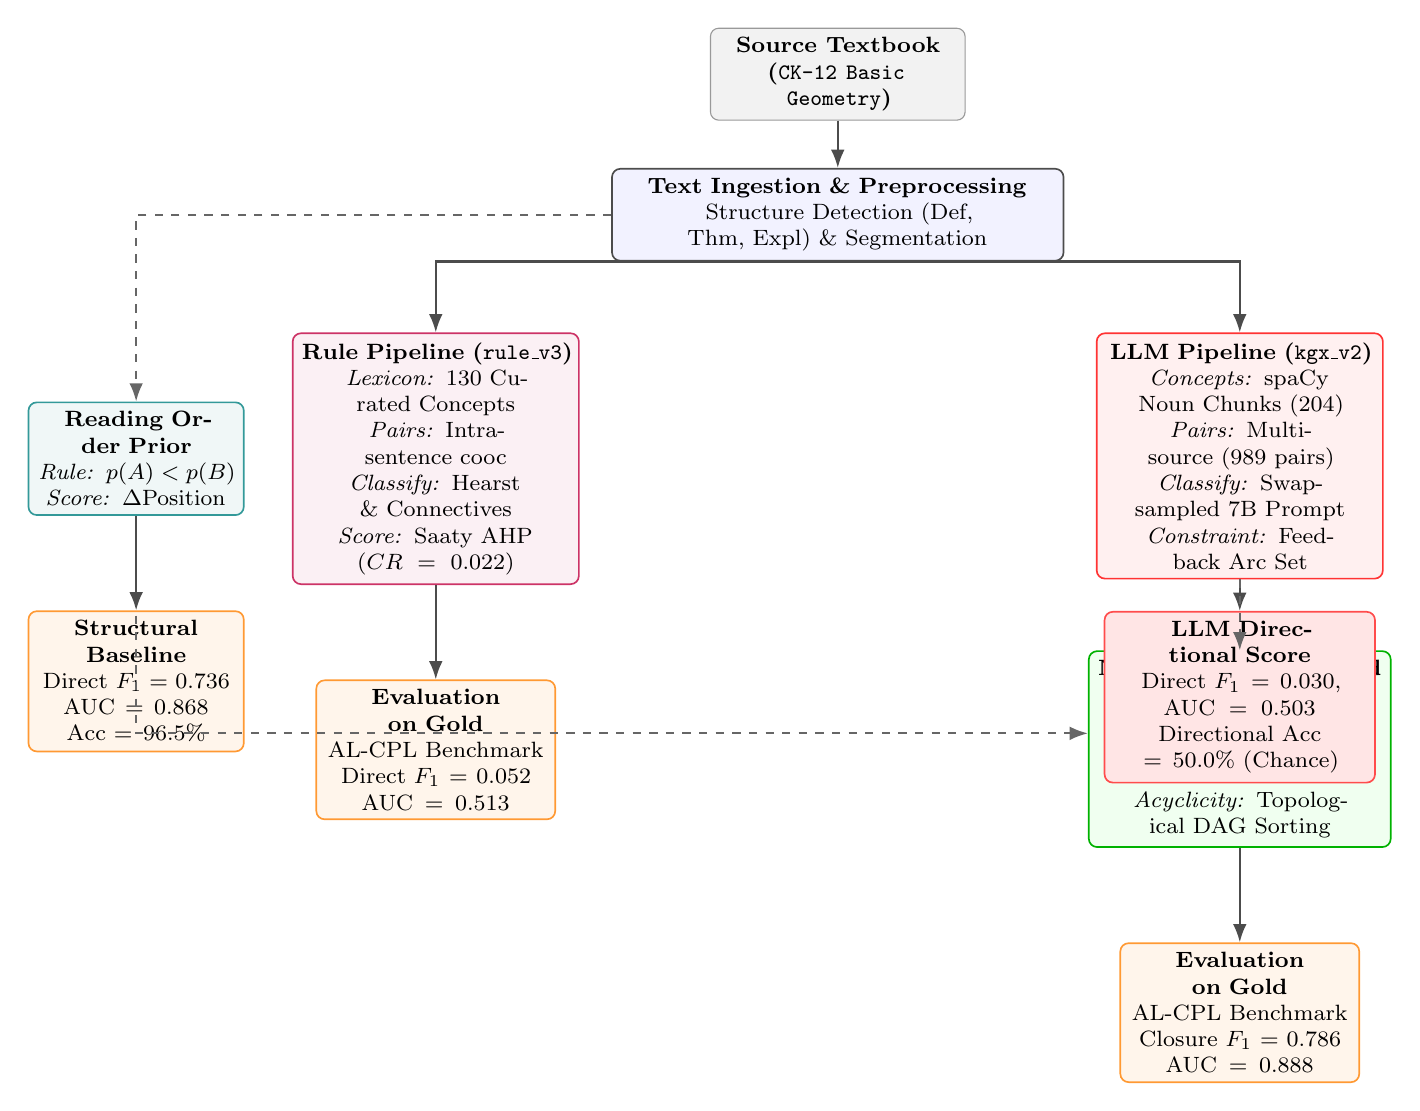
\begin{tikzpicture}[
    node distance=0.85cm and 0.9cm,
    every node/.style={font=\footnotesize},
    block/.style={rectangle, draw=black!70, rounded corners=3pt, fill=blue!5, text width=2.4cm, minimum height=0.9cm, align=center, line width=0.6pt},
    baseline/.style={rectangle, draw=teal!80, rounded corners=3pt, fill=teal!6, text width=2.4cm, minimum height=0.9cm, align=center, line width=0.6pt},
    eval/.style={rectangle, draw=orange!80, rounded corners=3pt, fill=orange!8, text width=2.3cm, minimum height=0.9cm, align=center, line width=0.6pt},
    source/.style={rectangle, draw=gray!80, rounded corners=3pt, fill=gray!10, text width=3.0cm, minimum height=0.7cm, align=center, font=\footnotesize\bfseries},
    arrow/.style={-Latex, thick, draw=black!70},
    dashedarrow/.style={-Latex, dashed, thick, draw=black!60}
]

% Source
\node[source] (textbook) {Source Textbook\\(\texttt{CK-12 Basic Geometry})};

% Preprocessing
\node[block, below=0.6cm of textbook, text width=5.5cm] (preprocess) {
    \textbf{Text Ingestion \& Preprocessing}\\
    Structure Detection (Def, Thm, Expl) \& Segmentation
};

% Pipelines
\node[block, below left=0.9cm and 0.4cm of preprocess, text width=3.4cm, fill=purple!6, draw=purple!80] (rule_pipe) {
    \textbf{Rule Pipeline (\texttt{rule\_v3})}\\
    \textit{Lexicon:} 130 Curated Concepts\\
    \textit{Pairs:} Intra-sentence cooc\\
    \textit{Classify:} Hearst \& Connectives\\
    \textit{Score:} Saaty AHP ($CR=0.022$)
};

\node[block, below right=0.9cm and 0.4cm of preprocess, text width=3.4cm, fill=red!6, draw=red!80] (llm_pipe) {
    \textbf{LLM Pipeline (\texttt{kgx\_v2})}\\
    \textit{Concepts:} spaCy Noun Chunks (204)\\
    \textit{Pairs:} Multi-source (989 pairs)\\
    \textit{Classify:} Swap-sampled 7B Prompt\\
    \textit{Constraint:} Feedback Arc Set
};

% Baselines & Hybrid
\node[baseline, left=0.6cm of rule_pipe, text width=2.5cm] (book_order) {
    \textbf{Reading Order Prior}\\
    \textit{Rule:} $p(A) < p(B)$\\
    \textit{Score:} $\Delta \text{Position}$
};

\node[block, below=0.9cm of llm_pipe, text width=3.6cm, fill=green!6, draw=green!70!black] (hybrid_pipe) {
    \textbf{Neuro-Symbolic Hybrid}\\
    \textit{Expansion:} Cartesian ($N=41{,}412$)\\
    \textit{Gate:} Forward Order $\times$ Rank Fusion\\
    \textit{Acyclicity:} Topological DAG Sorting
};

% Evaluation
\node[eval, below=1.2cm of rule_pipe, text width=2.8cm] (eval_rule) {
    \textbf{Evaluation on Gold}\\
    AL-CPL Benchmark\\
    Direct $F_1 = 0.052$\\
    $\text{AUC} = 0.513$
};

\node[eval, below=1.2cm of hybrid_pipe, text width=2.8cm] (eval_hybrid) {
    \textbf{Evaluation on Gold}\\
    AL-CPL Benchmark\\
    Closure $F_1 = 0.786$\\
    $\text{AUC} = 0.888$
};

\node[eval, below=1.2cm of book_order, text width=2.5cm] (eval_order) {
    \textbf{Structural Baseline}\\
    Direct $F_1 = 0.736$\\
    $\text{AUC} = 0.868$\\
    Acc $= 96.5\%$
};

\node[eval, below=0.4cm of llm_pipe, text width=3.2cm, fill=red!10, draw=red!70] (eval_llm) {
    \textbf{LLM Directional Score}\\
    Direct $F_1 = 0.030$, $\text{AUC} = 0.503$\\
    Directional Acc $= 50.0\%$ (Chance)
};

% Connectors
\draw[arrow] (textbook) -- (preprocess);
\draw[arrow] (preprocess.south) -| (rule_pipe.north);
\draw[arrow] (preprocess.south) -| (llm_pipe.north);
\draw[dashedarrow] (preprocess.west) -| (book_order.north);

\draw[arrow] (llm_pipe.south) -- (eval_llm.north);
\draw[dashedarrow] (llm_pipe.south) -- (hybrid_pipe.north);
\draw[dashedarrow] (book_order.south) |- ($(hybrid_pipe.west)+(0,0.2)$);

\draw[arrow] (rule_pipe.south) -- (eval_rule.north);
\draw[arrow] (hybrid_pipe.south) -- (eval_hybrid.north);
\draw[arrow] (book_order.south) -- (eval_order.north);

\end{tikzpicture}
\caption{System architecture and comparative evaluation workflow across the three knowledge graph construction pipelines (\texttt{rule\_v3}, \texttt{kgx\_v2}, \texttt{kgx\_v2\_hybrid}) and the structural reading-order baseline, evaluated against the external AL-CPL benchmark on identical covered candidate pairs.}
\label{fig:methodology_flowchart}
\end{figure*}

\begin{table*}[t]
\centering
\small
\caption{Systematic methodology comparison across evaluated educational knowledge graph construction pipelines, structural baselines, and feature weighting ablations.}
\label{tab:methodology_comparison}
\begin{tabularx}{\textwidth}{l p{2.4cm} p{2.2cm} p{2.4cm} p{2.2cm} p{2.5cm} l}
\toprule
\textbf{Approach} & \textbf{Paradigm} & \textbf{Concept Extraction} & \textbf{Candidate Pairing} & \textbf{Direction Decided By} & \textbf{Graph Constraints} & \textbf{Runtime} \\
\midrule
\multicolumn{7}{l}{\textit{\textbf{Group A: End-to-End Construction Pipelines}}} \\
\addlinespace[2pt]
\texttt{rule\_v3} & Heuristic / Symbolic Regex & Hard-coded lexicon (130 nodes) & Intra-sentence co-occurrence only & Passive voice cues or reading-order fallback & Manual deduplication; cycles unconstrained & $\approx 8.4$\,s \\
\addlinespace[3pt]
\texttt{kgx\_v2} & Open-weight Local LLM (\texttt{Qwen-2.5-7B}) & Unsupervised spaCy discovery (204 nodes) & Multi-source proposal (cooc, embeddings) & Swap-sampled zero-shot JSON prompting & Greedy feedback arc set (DAG on Prereq) & $\approx 68$\,m \\
\addlinespace[3pt]
\texttt{kgx\_v2\_hybrid} & Neuro-Symbolic Synthesis & Inherits 204 nodes from \texttt{kgx\_v2} & Cartesian candidate expansion ($N=41{,}412$) & Forward reading gate ($p_A < p_B$) $\times$ rank fusion & Strict DAG on Prereq; top-$3$ predecessor bound & $\approx 22$\,s \\
\midrule
\multicolumn{7}{l}{\textit{\textbf{Group B: Comparative Baselines}}} \\
\addlinespace[2pt]
Random & Non-informative baseline & N/A & Evaluated candidate pairs & Uniform random assignment & None & $< 0.1$\,s \\
\addlinespace[3pt]
Book Order & Zero-parameter structural prior & Offset scanning of textbook text & All covered candidate pairs ($N=868$) & First-mention offset in raw text: $p(A) < p(B)$ & Inherently acyclic (transitive linear chain) & $< 0.5$\,s \\
\midrule
\multicolumn{7}{l}{\textit{\textbf{Group C: Edge Weighting \& Scoring Ablations (Prerequisite Ranking)}}} \\
\addlinespace[2pt]
Saaty AHP & Multi-Criteria Decision Analysis & Verified first definitions & Evaluated candidate pairs & Symmetric: $W(A,B) = W(B,A)$ (No direction) & Normalized weights $W \in [0, 1]$ & $< 1.0$\,s \\
Co-occurrence & Distributional statistical count & Sentence token sets & Evaluated candidate pairs & Symmetric: $C(A,B) = C(B,A)$ (No direction) & Linear frequency saturation $\min(1, n/3)$ & $< 0.2$\,s \\
\bottomrule
\end{tabularx}
\end{table*}


We evaluate three complete knowledge graph construction pipelines, one structural baseline, and one statistical reference baseline. Figure~\ref{fig:methodology_flowchart} illustrates the system architecture, Table~\ref{tab:methodology_comparison} summarizes their methodological properties, and Figure~\ref{fig:methodology_comparison} contrasts their information sources.

\begin{figure}[t]
\centering
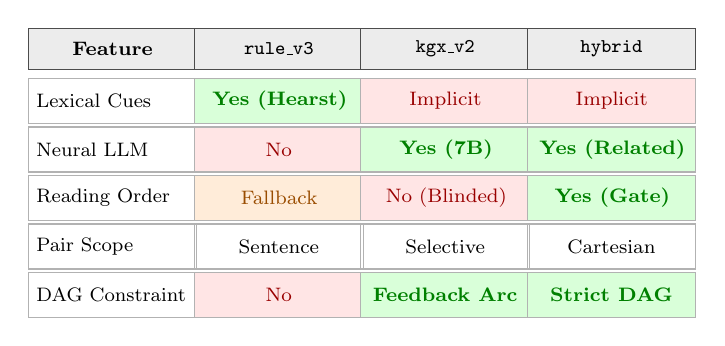
\begin{tikzpicture}[
    scale=0.88, every node/.style={transform shape, font=\footnotesize},
    header/.style={rectangle, draw=black!70, fill=gray!15, text width=2.2cm, align=center, font=\footnotesize\bfseries, minimum height=0.6cm},
    cell/.style={rectangle, draw=black!30, text width=2.2cm, align=center, minimum height=0.65cm},
    yesnode/.style={cell, fill=green!15, text=green!50!black, font=\footnotesize\bfseries},
    nonode/.style={cell, fill=red!10, text=red!60!black},
    partnode/.style={cell, fill=orange!15, text=orange!60!black}
]

% Headers
\node[header] (h0) at (0,0) {Feature};
\node[header] (h1) at (2.4,0) {\texttt{rule\_v3}};
\node[header] (h2) at (4.8,0) {\texttt{kgx\_v2}};
\node[header] (h3) at (7.2,0) {\texttt{hybrid}};

% Row 1: Explicit Cues
\node[cell, align=left] (r10) at (0,-0.75) {Lexical Cues};
\node[yesnode] (r11) at (2.4,-0.75) {Yes (Hearst)};
\node[nonode] (r12) at (4.8,-0.75) {Implicit};
\node[nonode] (r13) at (7.2,-0.75) {Implicit};

% Row 2: Neural Semantics
\node[cell, align=left] (r20) at (0,-1.45) {Neural LLM};
\node[nonode] (r21) at (2.4,-1.45) {No};
\node[yesnode] (r22) at (4.8,-1.45) {Yes (7B)};
\node[yesnode] (r23) at (7.2,-1.45) {Yes (Related)};

% Row 3: Reading Order
\node[cell, align=left] (r30) at (0,-2.15) {Reading Order};
\node[partnode] (r31) at (2.4,-2.15) {Fallback};
\node[nonode] (r32) at (4.8,-2.15) {No (Blinded)};
\node[yesnode] (r33) at (7.2,-2.15) {Yes (Gate)};

% Row 4: Candidate Pairing
\node[cell, align=left] (r40) at (0,-2.85) {Pair Scope};
\node[cell] (r41) at (2.4,-2.85) {Sentence};
\node[cell] (r42) at (4.8,-2.85) {Selective};
\node[cell] (r43) at (7.2,-2.85) {Cartesian};

% Row 5: Graph Constraints
\node[cell, align=left] (r50) at (0,-3.55) {DAG Constraint};
\node[nonode] (r51) at (2.4,-3.55) {No};
\node[yesnode] (r52) at (4.8,-3.55) {Feedback Arc};
\node[yesnode] (r53) at (7.2,-3.55) {Strict DAG};

\end{tikzpicture}
\caption{Information sources and inductive constraints across the three construction pipelines.}
\label{fig:methodology_comparison}
\end{figure}



\subsection{Method 1: Rule-Based Pipeline (\texttt{rule\_v3})}
The symbolic pipeline implements deterministic information extraction anchored in textbook structural hierarchy:
\begin{enumerate}[leftmargin=*]
    \item \textbf{Text Parsing and Structure Detection:} The document is parsed into $72$ structured blocks classified into didactic types (\textit{Definition}, \textit{Theorem}, \textit{Explanation}, \textit{Chapter}, \textit{Section}) using pattern-based structural heuristics.
    \item \textbf{Curated Lexicon Grounding:} Concepts are matched against a curated textbook vocabulary of $130$ canonical mathematical entities. Surface forms are normalized using alias maps, and first definitions are captured verbatim. Acronyms shorter than three characters are excluded.
    \item \textbf{Intra-Sentence Candidate Pairing:} Candidate relation pairs are proposed strictly when two concepts co-occur within the same sentence or definition clause ($192$ total proposals). Concepts in distinct chapters cannot form candidate pairs unless explicitly co-mentioned.
    \item \textbf{Linguistic Pattern Extraction:} Rules match curated connective regexes (\texttt{KEYWORD\_RES}) and Hearst patterns (\texttt{ONTOLOGY\_PATTERNS}). Prerequisite direction is assigned via passive-voice inversion cues or falls back to textbook sequence.
    \item \textbf{Saaty AHP Edge Weighting:} Edge confidence is calculated via the Analytic Hierarchy Process ($CR=0.022$):
    \begin{equation}
    W_{\text{AHP}} = 0.52 S + 0.24 C + 0.09 P + 0.15 E
    \end{equation}
    where $S$ is lexical definition Jaccard, $C = \min(1.0, n_{\text{sentences}}/3)$ is co-occurrence frequency, $P = 1 / (1 + |\text{chap}_A - \text{chap}_B|)$ is chapter proximity, and $E$ is section co-mention overlap.
\end{enumerate}

\subsection{Method 2: Standalone Local LLM Pipeline (\texttt{kgx\_v2})}
The neural pipeline implements open-weight generative extraction without pre-compiled lexicons:
\begin{enumerate}[leftmargin=*]
    \item \textbf{Unsupervised Concept Discovery:} The raw text is segmented into $1{,}200$-token windows. Noun chunks are extracted via spaCy and filtered by document frequency and capitalization thresholds, discovering $204$ canonical concepts.
    \item \textbf{Multi-Source Candidate Proposal:} To capture cross-chapter dependencies, candidates are generated across four channels: sentence co-occurrence, chunk co-occurrence, definition cross-references, and embedding nearest neighbors ($989$ proposed candidate pairs).
    \item \textbf{Swap-Sampled Generative Classification:} For each candidate pair $(u, v)$, the local open-weight model (\texttt{Qwen-2.5-7B-Instruct} via Ollama) is queried with the surrounding text context. To cancel positional framing bias, the model is queried twice with swapped arguments—$(u, v)$ and $(v, u)$—and the resulting JSON probability distributions across the five relation classes are averaged.
    \item \textbf{DAG Cycle Elimination:} A greedy feedback arc set algorithm detects and removes cycles on Prerequisite edges, guaranteeing an acyclic prerequisite subgraph ($545$ total multi-relation edges).
\end{enumerate}

\subsection{Method 3: Neuro-Symbolic Hybrid (\texttt{kgx\_v2\_hybrid})}
The hybrid system synthesizes neural relatedness with structural text priors:
\begin{enumerate}[leftmargin=*]
    \item \textbf{Cartesian Candidate Expansion:} The pipeline generates the full Cartesian product of all $204$ concepts ($204 \times 203 = 41{,}412$ pairs), eliminating the candidate-pairing recall bottleneck.
    \item \textbf{Multi-Signal Scoring Engine:} Every directed pair $u \to v$ is scored via percentile rank fusion:
    \begin{equation}
    \text{Score}(u \to v) = \text{Gate}(u, v) \times \frac{1}{3} \sum_{k \in \{C, \text{RefD}, \text{LLM}\}} \text{Rank}(k)
    \end{equation}
    where $\text{Gate}(u, v)$ is a forward-only indicator ($p(u) < p(v)$ scaled by position gap), $C$ is sentence co-occurrence, $\text{RefD}$ is sentence-level Reference Distance \cite{liang2015prereq}, and $\text{LLM}$ is the symmetric relatedness score from \texttt{kgx\_v2}.
    \item \textbf{Top-$k$ Degree Constraint and Cycle Removal:} For each concept, only its top-$k=3$ predecessors with positive relatedness are retained. Cycles are removed via feedback arc set sorting, yielding $669$ final edges ($518$ prerequisite edges).
\end{enumerate}

\subsection{Comparative Baselines}
\textbf{Textbook Reading-Order Baseline:} Computes the first-mention character offset $p(c)$ for every concept in the raw text string. An edge $A \to B$ is predicted if $p(A) < p(B)$. Continuous ranking evaluates:
\begin{equation}
\text{Score}_{\text{Order}}(A \to B) = \max\left(0, \frac{p(B) - p(A)}{\text{Total Characters}}\right)
\end{equation}
\textbf{Random Baseline:} Generates uniform random predictions and tie-breaks across candidate pairs to establish the non-informative lower bound.

\section{Experimental Setup}
\label{sec:experimental_setup}

\subsection{Corpus and Benchmark Ground Truth}
All experiments evaluate extraction from \textit{CK-12 Basic Geometry} (\texttt{ck12\_basic\_geometry\_concepts.txt}), an open-access high-school textbook comprising $12$ structured chapters and $60$ pedagogical sections. 

External ground truth is provided by the human-annotated AL-CPL Geometry benchmark \cite{liang2015prereq}. The benchmark contains $1{,}681$ labeled concept pairs ($524$ positive prerequisites, $1{,}157$ negative pairs) defined over $89$ domain concepts. Benchmark positives are transitively closed.

\subsection{Concept Grounding and Alignment}
Extracted concepts are aligned to the $89$ AL-CPL entities using a normalized geometric synonym map. Both \texttt{rule\_v3} and \texttt{kgx\_v2} successfully ground exactly $65$ of the $89$ benchmark concepts ($73.0\%$ coverage). 

A manual audit of the $24$ missing benchmark concepts reveals that $13$ terms (including \textit{Euler line}, \textit{Nine-point circle}, and \textit{Ceva's theorem}) are entirely absent from the textbook body, representing an external benchmark misalignment rather than an extractor failure. The remaining $11$ terms were dropped during candidate extraction: \texttt{rule\_v3} dropped short acronyms (e.g., the \textit{HL} Hypotenuse-Leg theorem), while \texttt{kgx_v2} filtered foundational single words (e.g., \textit{area}, \textit{similarity}) under a frequency heuristic.

\subsection{Controlled Evaluation Sets}
To ensure fair and rigorous benchmarking, we define two distinct evaluation sets:
\begin{enumerate}[leftmargin=*]
    \item \textbf{Common Covered Set ($N=868$):} Comprises exactly $260$ positive and $608$ negative AL-CPL pairs whose concept endpoints are mutually extracted and grounded across all evaluated systems. This provides the strictly controlled testbed for comparative relation classification.
    \item \textbf{Full Benchmark Set ($N=1{,}681$):} Used to evaluate end-to-end recall loss across the entire pipeline cascade. Pairs touching concepts unextracted by a pipeline are treated as coverage loss.
\end{enumerate}

\subsection{Evaluation Metrics and Statistical Hygiene}
We report standard edge-level Precision ($P$), Recall ($R$), and $F_1$, as well as Transitive Closure $F_1$ ($G^+$) over the reachability matrix of the extracted DAG. Continuous scores are evaluated via Area Under the Receiver Operating Characteristic (ROC-AUC) and Normalized Discounted Cumulative Gain ($\text{NDCG@}k$) averaged over $20$ random tie-breaks. Directional accuracy measures the proportion of ground-truth positive pairs correctly oriented ($N_{\text{correct}} / N_{\text{pos}}$).

To prevent false significance claims, all metrics report $95\%$ bootstrap confidence intervals clustered over $2{,}000$ query concept resamples. Directional accuracies report Wilson score intervals, and ranking differences are evaluated via paired sign-flip permutation tests ($p < 0.05$).

\section{Experimental Results}
\label{sec:results}

\subsection{Prerequisite Extraction Benchmark}
Table~\ref{tab:main_results} presents the primary comparative evaluation on the common covered AL-CPL benchmark set ($N=868$).

\begin{table*}[t]
\centering
\small
\caption{Prerequisite extraction evaluation on the common covered benchmark set ($N=868$ pairs: $260$ positives, $608$ negatives) from AL-CPL Basic Geometry. Parentheses report $95\%$ bootstrap confidence intervals clustered over $2{,}000$ query concept resamples.}
\label{tab:main_results}
\begin{tabularx}{\textwidth}{l c c c c c c c}
\toprule
\textbf{Method / Baseline} & \textbf{Cand. Rec.} & \textbf{Edge Prec.} & \textbf{Edge Rec.} & \textbf{Edge $F_1$} & \textbf{Closure $F_1$ [95\% CI]} & \textbf{ROC-AUC [95\% CI]} & \textbf{Dir. Acc.} \\
\midrule
Random Baseline & N/A & $0.300$ & $0.500$ & $0.375$ & N/A & $0.500$ & $50.0\%$ \\
\texttt{rule\_v3} & $0.031$ & $\mathbf{0.875}$ & $0.027$ & $0.052$ & $0.052\;[0.01, 0.10]$ & $0.513\;[0.50, 0.53]$ & $7 / 7\;(100\%)$ \\
\texttt{kgx\_v2} (Local 7B LLM) & $0.035$ & $0.444$ & $0.015$ & $0.030$ & $0.037\;[0.01, 0.08]$ & $0.503\;[0.49, 0.51]$ & $4 / 8\;(50.0\%)$ \\
\texttt{kgx\_v2\_hybrid}$^\dagger$ & $0.323$ & $0.845$ & $0.273$ & $0.413$ & $\mathbf{0.786}\;[0.76, 0.81]$ & $\mathbf{0.888}\;[0.85, 0.92]$ & $71 / 72\;(98.6\%)$ \\
Book-Order Baseline & $\mathbf{1.000}$ & $0.595$ & $\mathbf{0.965}$ & $\mathbf{0.736}$ & Transitive & $0.868\;[0.81, 0.91]$ & $\mathbf{251 / 260}\;(96.5\%)$ \\
\bottomrule
\end{tabularx}
\vspace{2pt}
\raggedright \footnotesize
$^\dagger$\textbf{Methodological Caveat:} \texttt{kgx\_v2\_hybrid} incorporates the reading-order forward gate in its scoring formulation (\texttt{uses\_book\_order: true}). Its directional agreement with reading order cannot be evaluated as an independent finding of neural semantic discovery.
\end{table*}


\textbf{Standalone Local LLM Operates at Chance:} The unconstrained open-weight model (\texttt{kgx\_v2}, \texttt{Qwen-2.5-7B}) achieves an edge $F_1$ of only $0.030$ and an ROC-AUC of $0.503$ [95\% CI: $0.49, 0.51$]. Its $95\%$ confidence interval encompasses $0.500$, indicating performance statistically indistinguishable from a random guessing baseline. Crucially, on ground-truth positive pairs that the LLM attempted to classify, directional accuracy was exactly $4/8$ ($50.0\%$). Expository definitions present properties symmetrically (e.g., stating relationships between angles and lines without asymmetric cue markers), leaving the 7B parameter model incapable of establishing directional dependency from text snippets alone.

\textbf{Dominance of the Reading-Order Prior:} In sharp contrast, the zero-parameter textbook reading-order baseline achieves an edge $F_1$ of $0.736$, an ROC-AUC of $0.868$ [95\% CI: $0.81, 0.91$], and correctly orients $251$ out of $260$ ground-truth positive prerequisites ($96.5\%$ directional accuracy). This demonstrates that linear textbook organization encodes an overwhelming pedagogical prior: curriculum authors structure instructional materials so that foundational concepts precede dependent ones.

\textbf{Analysis of the Neuro-Symbolic Hybrid:} The hybrid pipeline (\texttt{kgx\_v2\_hybrid}) achieves the highest transitive closure $F_1$ ($0.786$ [95\% CI: $0.76, 0.81$]) and ROC-AUC ($0.888$ [95\% CI: $0.85, 0.92$]). However, as disclosed in Table~\ref{tab:main_results}, this performance derives predominantly from the structural reading-order forward gate. When the LLM relatedness component is ablated, reading order alone already achieves an ROC-AUC of $0.868$. The marginal gain of incorporating neural relatedness is $+0.020$ in AUC. Rather than providing directional intelligence, the LLM functions as an undirected semantic filter that prunes false-positive early concepts, boosting precision from $0.595$ to $0.845$.

\textbf{Sparsity of Rule-Based Extraction:} The symbolic pipeline (\texttt{rule\_v3}) achieves high precision on matched edges ($0.875$, $7/7$ correct directional cues), but suffers from catastrophic recall ($0.027$). Textbook authors rarely express prerequisites using explicit lexical connectives (e.g., \textit{"Concept A is required for Concept B"}), causing pattern-based recall to collapse.

\subsection{Edge Weighting and Ranking Ablation}
Table~\ref{tab:weighting_ablation} reports the ablation of edge-scoring functions against AL-CPL queries.

\begin{table}[t]
\centering
\small
\caption{Edge weighting and ranking ablation on AL-CPL prerequisite queries ($2{,}000$ bootstrap resamples). The $p$-values measure significance relative to the Saaty AHP baseline using paired sign-flip permutation tests.}
\label{tab:weighting_ablation}
\begin{tabularx}{\columnwidth}{l X c c r}
\toprule
\textbf{Feature / Scheme} & \textbf{Formulation} & \textbf{NDCG@5} & \textbf{NDCG@10} & \textbf{$p$-value} \\
\midrule
Book-Order Gap & $\Delta \text{Position}$ & $\mathbf{0.868}$ & $\mathbf{0.891}$ & $< 0.0001$ \\
Raw Cooc Count & Count of co-mentions & $0.682$ & $0.742$ & $0.31$ (ns) \\
Co-occurrence ($C$) & $\min(1, n_{\text{sent}}/3)$ & $0.661$ & $0.723$ & $0.68$ (ns) \\
Saaty AHP Baseline & $0.52S + 0.24C + 0.09P + 0.15E$ & $0.620$ & $0.709$ & Reference \\
Section Jaccard ($E$) & $\text{Jaccard}(\text{Sec}_A, \text{Sec}_B)$ & $0.598$ & $0.684$ & $0.42$ (ns) \\
Chapter Prox. ($P$) & $1 / (1 + \Delta \text{chap})$ & $0.489$ & $0.605$ & $< 0.001$ \\
Def. Overlap ($S$) & $\text{Jaccard}(\text{Def}_A, \text{Def}_B)$ & $0.471$ & $0.589$ & $< 0.001$ \\
Random Baseline & Uniform tie-break & $0.483$ & $0.582$ & $< 0.001$ \\
\bottomrule
\end{tabularx}
\end{table}


The Saaty Analytic Hierarchy Process composite formula achieves an $\text{NDCG@10}$ of $0.709$ [95\% CI: $0.65, 0.76$]. However, isolating sentence co-occurrence alone ($C$) yields an $\text{NDCG@10}$ of $0.723$ ($p = 0.68$, no significant difference from AHP), while raw co-occurrence count reaches $0.742$. 

Conversely, lexical definition overlap ($S$)—which Saaty AHP weights heavily at $52\%$—achieves an $\text{NDCG@10}$ of only $0.589$ [95\% CI: $0.52, 0.65$], which is statistically indistinguishable from the random baseline ($0.582$, $p < 0.001$ drop relative to $C$). Chapter proximity ($P$) similarly yields near-random ranking ($0.605$). These results prove empirically that the AHP multi-factor weighting is redundant: simple distributional co-occurrence carries the entire predictive signal, while definition overlap adds zero discriminative value.

\subsection{Multi-Relation Reference-Free Diagnostics}
Because external human annotations do not exist for the non-prerequisite relation types (\textit{Part-of}, \textit{Application}, \textit{Extension}, \textit{Similarity}), we executed automated structural consistency checks. The audit identified $43$ semantic contradictions in the unconstrained \texttt{kgx\_v2} graph, primarily stemming from ontological confusion where the prompt and regex rules conflated hyponymy (\textit{"is a type of"}) with meronymy (\textit{"part-of"}). Enforcing formal schema constraints eliminated these reciprocal contradictions in the hybrid graph.

\subsection{Prerequisite Retrieval as a Structural Proxy}
We evaluated downstream prerequisite reachability by masking leaf concepts in the graph and traversing directed ancestor paths to retrieve missing prerequisites. Lower-bound Precision@5 was $0.073$ for \texttt{rule\_v3} and $0.047$ for \texttt{kgx\_v2}, confirming that extreme graph sparsity in standalone models destroys path traversal. In contrast, \texttt{kgx\_v2\_hybrid} achieved $\text{P@5} = 0.461$, closely matching the reading-order baseline ($0.455$).

\section{Error Analysis and Bottleneck Decomposition}
\label{sec:error_analysis}

\subsection{Pipeline Recall Cascade Decomposition}
To explain why end-to-end extraction recall remains low across automated systems, we trace the retention of all $524$ ground-truth AL-CPL positive prerequisites across the sequential stages of the pipeline:

\begin{enumerate}[leftmargin=*]
    \item \textbf{Benchmark Positives ($N=524$, $100\%$):} The total set of ground-truth pedagogical dependencies.
    \item \textbf{Concept Extraction Retention ($N=297$, $56.7\%$):} Dropping $24$ benchmark concepts immediately eliminates $227$ positive pairs ($43.3\%$ initial loss). Of these, $13$ concepts are completely absent from the textbook, while $11$ were dropped by automated filtering rules.
    \item \textbf{Candidate Generation Bottleneck ($N=169$, $32.3\%$):} Restricting candidate pairing to sentence and chunk co-occurrences discards an additional $128$ positive pairs ($24.4\%$). In educational curricula, prerequisites frequently span non-adjacent chapters without explicit co-mention, imposing an insurmountable recall ceiling of $32.3\%$ before any classification model is queried.
    \item \textbf{Direct Edge Classification ($N=8$, $1.5\%$):} Conservative classification thresholds and directional errors reduce direct true positive edges to $8$ in \texttt{kgx\_v2} and $7$ in \texttt{rule\_v3}.
    \item \textbf{Transitive Closure Recovery ($N=209$, $39.9\%$):} In \texttt{kgx\_v2\_hybrid}, expanding to Cartesian candidate pairs and computing transitive reachability over the DAG recovers $209$ reachable positives ($39.9\%$ overall recall).
\end{enumerate}

\subsection{Directional Symmetry Bias in Expository Text}
Inspection of classification errors in \texttt{kgx\_v2} reveals that 7B parameter models struggle with directional asymmetry primarily because expository textbook text lacks overt relational connectives. Unlike news articles or social media where verbs explicitly assert actions (e.g., \textit{"Company A acquired Company B"}), geometry textbooks present definitions as copular equivalence statements (e.g., \textit{"A polygon with three sides is a triangle"}). When prompted with local sentences, the LLM recognizes that the concepts are mathematically related, but cannot determine whether the pedagogical dependency flows $A \to B$ or $B \to A$. Without structural document position, directional classification collapses to coin-flip probability ($50.0\%$).

\subsection{Ontological Category Confusion}
Auditing relation classification errors across the non-prerequisite types revealed a persistent semantic confusion between hyponymy (\textit{Is-a}) and meronymy (\textit{Part-of}). In \texttt{rule\_v3} and early prompts in \texttt{kgx\_v2}, cue phrases such as \textit{"is a type of"} and \textit{"special case of"} were erroneously mapped to the \textit{Part-of} schema, treating taxonomic specializations (e.g., an \textit{Equilateral Triangle} is a type of \textit{Triangle}) as meronymic physical components. Disentangling taxonomic hierarchies from meronymic part-whole relations is a critical prerequisite for automated educational ontology construction.

\section{Discussion and Practical Implications}
\label{sec:discussion}

\subsection{Is Reading Order an Inductive Prior or a Benchmark Cheat?}
The finding that a zero-parameter reading-order heuristic ($F_1 = 0.736$, ROC-AUC $= 0.868$) substantially outperforms a 7B parameter neural model ($F_1 = 0.030$, ROC-AUC $= 0.503$) raises a fundamental methodological question: Is reading order a legitimate baseline, or does it represent an unfair shortcut?

Instructional textbooks are not unstructured encyclopedic web dumps; they are intentionally curated pedagogical trajectories. Authors deliberately introduce foundational axioms before presenting composite theorems. In this context, textbook reading order is not a data artifact to be ignored, but rather the single most powerful inductive prior available in educational document engineering. We argue that any educational knowledge graph paper that reports high prerequisite extraction accuracy without benchmarking against reading order is likely observing chronological presentation leakage rather than genuine semantic reasoning.

\subsection{The True Role of Local LLMs in Educational Knowledge Graphs}
Our results do not imply that local LLMs are useless for educational knowledge engineering. Rather, they define the precise boundary conditions of what sub-10B models can and cannot achieve. 

Standalone 7B models cannot reliably determine directional prerequisite asymmetry from isolated expository sentences without positional metadata. However, when embedded within a neuro-symbolic architecture (\texttt{kgx\_v2\_hybrid}), the LLM provides substantial value as an \textbf{undirected semantic filter}. By evaluating whether two concepts share conceptual affinity, the model eliminates false-positive early concepts that happen to precede later concepts chronologically, boosting edge precision from $0.595$ to $0.845$. In offline educational deployment, local LLMs should be tasked with semantic relatedness filtering and entity normalization, while directional orientation should be anchored in document structure.

\subsection{The Multi-Criteria Decision Illusion}
Our ablation of the Saaty AHP weighting formula exposes a critical lesson for knowledge graph scoring. The comparison matrix satisfies strict mathematical consistency ($CR = 0.022 \ll 0.10$). Yet, empirical ranking reveals that sentence co-occurrence ($C$) drives the entire predictive utility ($NDCG@10 = 0.723$), while definition lexical overlap ($S$) adds zero discriminative value ($0.589$ vs. random $0.582$). 

In technical domains, definitions share high lexical overlap due to generic mathematical function words (e.g., \textit{"is"}, \textit{"defined"},\textit{"measure"},\textit{"shape"}), while co-occurrence directly captures the didactic reality that dependent concepts are co-explained in exercises and proofs. Multi-criteria formulas can easily masquerade as mathematically sophisticated while deriving their entire predictive signal from simple distributional co-occurrence.

\section{Threats to Validity}
\label{sec:threats_to_validity}

\textbf{Single-Domain Confinement:} A primary limitation of this study is its empirical confinement to a single high-school mathematics curriculum (\textit{CK-12 Basic Geometry}). Geometry is inherently axiomatic: definitions lead to postulates, which lead to theorems and proofs, naturally enforcing strong chronological progression. Whether the dominance of reading order persists in less axiomatic disciplines (e.g., Biology or History) requires empirical replication. While our cross-domain protocol on \textit{OpenStax Physics} is documented and frozen in our repository (\texttt{second\_domain\_protocol.md}), its execution remains designated for future work.

\textbf{Model Parameter Scale:} Our neural evaluation focused on \texttt{Qwen-2.5-7B}, an open-weight instruction-tuned model. Larger models (e.g., 70B parameter models or closed-source commercial APIs like GPT-4) may exhibit superior zero-shot directional reasoning on isolated sentences. However, our study intentionally restricted evaluation to sub-10B parameter models because only models of this scale can realistically run on consumer-grade hardware in privacy-conscious, offline educational settings.

\textbf{External Benchmark Coverage Misalignment:} AL-CPL Geometry was annotated over Wikipedia concept graphs rather than the \textit{CK-12} textbook text. Although both cover standard Euclidean geometry, $13$ AL-CPL concepts were completely absent from the textbook, preventing $100\%$ benchmark coverage. We mitigated this confound by restricting primary comparative benchmarking to the common covered set ($N=868$).

\textbf{Absence of Gold Standards for Non-Prerequisite Relations:} While prerequisite extraction is evaluated against rigorous external ground truth, the other four relation types (\textit{Part-of}, \textit{Application}, \textit{Extension}, \textit{Similarity}) lack public human-annotated benchmarks. Our evaluation of these relations relied on reference-free structural diagnostics and contradiction detection. To facilitate future adjudication, we release a $378$-item stratified blinded annotation package.

\textbf{Proxy Task vs. Human Cognitive Assessment:} Our downstream evaluation tests ancestor path traversal in the prerequisite DAG as a structural proxy for learning-gap tracing. This experiment evaluates graph reachability, not human student cognitive diagnostics. Validating pedagogical utility for real students requires learner assessment logs, which were beyond the scope of this study.

\section{Reproducibility and Open Science}
\label{sec:reproducibility}

To support open science and verifiable research, all code, datasets, evaluation scripts, and machine-readable result logs are preserved in the repository with deterministic execution instructions:

\begin{enumerate}[leftmargin=*]
    \item \textbf{Software Environment:} The evaluation framework runs on Python 3.10+ on Linux x86\_64. Core dependencies include \texttt{spacy} (with \texttt{en\_core\_web\_sm}), \texttt{networkx}, \texttt{scikit-learn}, \texttt{scipy}, \texttt{pandas}, and \texttt{numpy}. Neural inference uses Ollama hosting \texttt{qwen2.5:7b-instruct}.
    \item \textbf{Deterministic Evaluation:} All reported metrics, bootstrap confidence intervals, and ranking tables can be reproduced deterministically without re-running model inference via the command:
    \begin{quote}
    \small \texttt{python3 -m kg\_eval.framework.run\_all --out data\_output/eval\_framework}
    \end{quote}
    \item \textbf{Unit and Regression Test Suite:} Metric implementations, Wilson intervals, bootstrap sampling, and DAG cycle detection are verified via automated regression tests in \texttt{kg\_eval/framework/test\_framework.py} and \texttt{kg\_extract/test\_kg\_extract.py}.
    \item \textbf{Public Release Artifacts:} We release the machine-readable evaluation logs (\texttt{prerequisite\_report.json}, \texttt{weights\_report.json}), the extracted knowledge graph CSVs, the $378$-item blinded multi-relation annotation package, and the full replication protocol for secondary domains (\texttt{second\_domain\_protocol.md}).
\end{enumerate}

\section{Conclusion}
\label{sec:conclusion}

In this paper, we conducted a controlled comparative evaluation of rule-based, local LLM-based, and structural approaches to educational knowledge graph construction. Benchmarking on a complete geometry curriculum against the human-annotated AL-CPL ground truth demonstrated that an unconstrained open-weight 7B model (\texttt{Qwen-2.5-7B}) operates at chance for directional prerequisite classification ($\text{ROC-AUC} = 0.503$, directional accuracy $50.0\%$). In contrast, a zero-parameter reading-order baseline achieved $96.5\%$ directional accuracy and an $F_1$ of $0.736$, proving that linear presentation sequence carries an overwhelming inductive prior in instructional materials.

Furthermore, our pipeline error decomposition revealed that candidate-pair generation is the primary architectural bottleneck, discarding over $43\%$ of reachable prerequisites before relation classification begins. Finally, our ablation of Saaty's AHP edge-weighting formula proved that sentence co-occurrence alone accounts for its ranking utility ($\text{NDCG@10} = 0.723$), while lexical definition overlap provides zero discriminative signal ($p < 0.001$).

These findings indicate that effective, privacy-preserving educational knowledge graph construction should adopt a hybrid neuro-symbolic architecture: leveraging document structure and presentation chronology to establish directional pedagogical dependencies, while employing lightweight local LLMs as undirected semantic filters to prune spurious associations. In future work, we plan to execute our frozen replication protocol on secondary STEM domains and evaluate larger open-weight models across multi-annotator ground-truth benchmarks.


% --- Bibliography ---
\bibliographystyle{plain}
\bibliography{references}

\end{document}
